\documentclass[12pt, a4paper, oneside]{memoir}
\chapterstyle{lyhne}

\usepackage[a4paper,width=150mm,top=25mm,bottom=25mm,nomarginpar]{geometry}

\usepackage[pdfauthor={OffCourse Staff},
            pdfcreator={OffCourse Staff under CC BY-SA 4.0},
            pdftitle={PYNQ USB Setup Reference},
            pdfkeywords={PYNQ PYNQ-Z2 pynq pynq-z2 TUL tul usb programming offcourse},
            pdfsubject={Setup to programming a TUL PYNQ-Z2 over USB}]{hyperref}

\usepackage{textcomp}
\usepackage[utf8]{inputenc}
\usepackage[table]{xcolor}
\usepackage{colortbl}
\usepackage[english]{babel}
\usepackage[english]{isodate}
\usepackage{lmodern}
\usepackage[T1]{fontenc}
\usepackage{wrapfig}
\usepackage{tcolorbox}
\usepackage{fancyhdr}
\pagestyle{fancy}
\makepagestyle{fancy}
\usepackage{minted}
\tcbuselibrary{minted}
\usepackage{tikz}
\usetikzlibrary{circuits.logic.US}
\usepackage{multirow}
\usepackage{graphfig}
\usepackage{graphicx}
\usepackage{circuitikz}
\usepackage{tikz-timing}
\usetikztiminglibrary{either}
\usepackage{svg}
\usepackage{bookmark}
\usepackage{caption}
\usepackage{subcaption}
\usepackage{titling}
\usepackage{enumitem}

\setlength{\marginparwidth}{2cm}
\usepackage[colorinlistoftodos,prependcaption]{todonotes}
\captionsetup{belowskip=0pt}

\newcolumntype{Y}{>{\centering\arraybackslash}X}

\newcommand{\attention}[1]{\begin{center}\colorbox{attention}{\textbf{#1}}\end{center}}
\renewcommand{\lnot}{\textasciitilde{}}

\begin{document}
\setlength{\beforechapskip}{-20pt}
\fancypagestyle{plain}{%
  \fancyhead[L]{By Student Assistants}
  \fancyhead[C]{\textbf{PYNQ \textsc{USB} Setup Reference}}
  \fancyhead[R]{CC BY-SA 4.0}
}

\fancyhead[L]{By Student Assistants}
\fancyhead[C]{\textbf{PYNQ \textsc{USB} Setup Reference}}
\fancyhead[R]{CC BY-SA 4.0}

\definecolor{attention}{cmyk}{0,0,0.4,0}
\definecolor{logicblue}{cmyk}{0.27,0.01,0,0.06}
\definecolor{gtkgreen}{rgb}{32,32,112}
\colorlet{tbDGrn}{white!40!green}
\colorlet{tbBlu}{white!60!blue}
\colorlet{tbRed}{white!55!red}

\chapter*{Setting up the PYNQ}
Before you can even try to program the PYNQ board over \textsc{usb}, you must first configure the hardware of the board.
Confirm both the \textbf{POWER} and \textbf{JTAG} selectors are set correctly.
Afterwards connect the PYNQ to your computer with the USB cable. The \textbf{red light} should come on immediatly. The \textbf{green light} should not come on by itself! It should only turn on after programming the PYNQ.
\begin{figure}[H]
  \centering
  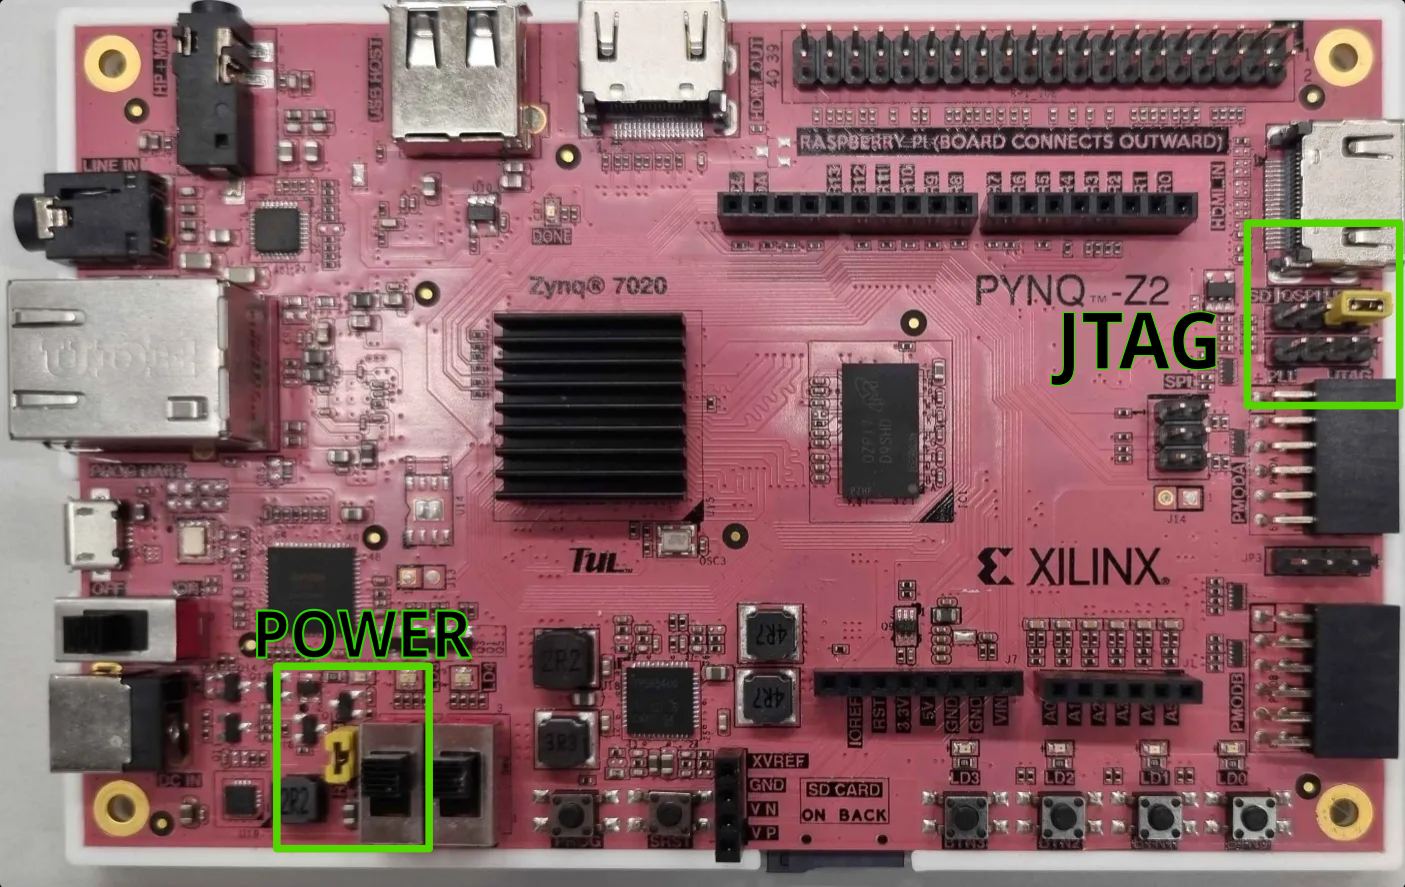
\includegraphics[width=\linewidth]{PYNQ_1_HIGH.png}
  \caption{PYNQ Board Selector Locations}
\end{figure}
\begin{figure}
  \centering
  \begin{tabular}{cc}
    \textbf{POWER Selector} & \textbf{JTAG Selector} \\
    Set to \textsc{usb} & Set to \textsc{jtag} \\
    \raisebox{116pt}{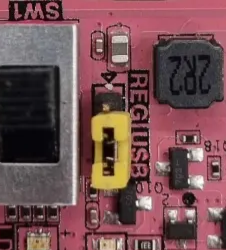
\includegraphics[width=150pt,angle=180]{PYNQ_POWER_CROP.png}} & 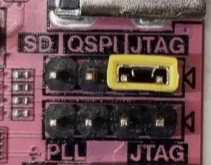
\includegraphics[width=150pt]{PYNQ_JTAG_CROP.png} \\
  \end{tabular}
\end{figure}

\pagebreak
\chapter*{Using the PYNQ from a VirtualBox Virtual Machine}
\begin{enumerate}[leftmargin=*]
    \item Boot the Virtual Machine and wait for the login page.
    \item After logging in, go to the \textbf{Devices} menu top-left and tick \textbf{USB$\rightarrow$Xilinx TUL[0700]} %PIC 3
    \item To verify the connection from the VM to the PYNQ, you can open the terminal and type \texttt{lsusb} then enter. The result should include a \textbf{FT2232 Dual UART}.
    \item \textit{Redo these steps everytime you start or reboot the Virtual Machine.}
\end{enumerate}

\begin{figure}[H]
  \centering
  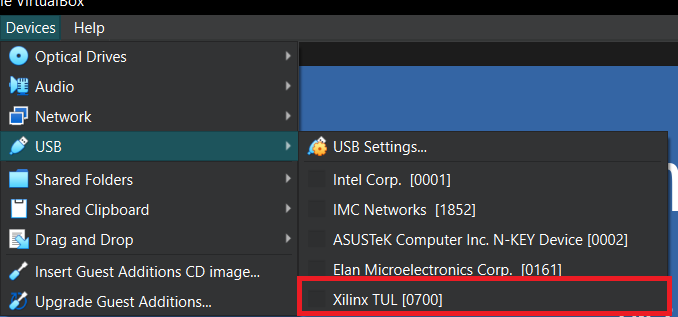
\includegraphics[width=0.75\linewidth]{CA_3.png}
  \caption{\texttt{Allow access to the PYNQ.}}
\end{figure}

\begin{figure}[H]
  \centering
  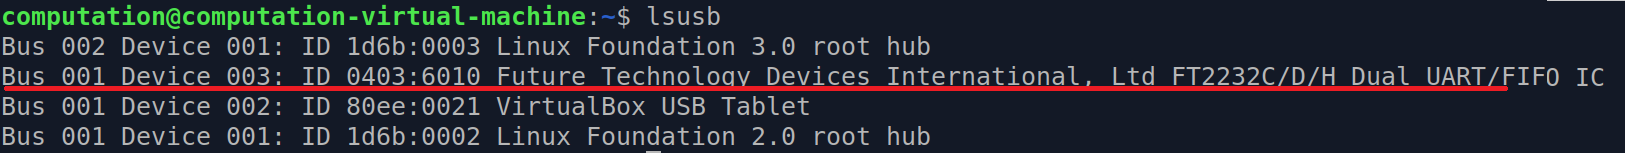
\includegraphics[width=\linewidth]{CA_4.png}
  \caption{\texttt{lsusb} output.}
\end{figure}
\section*{Troubleshooting}
\begin{table}[H]
  \centering
  \begin{tabular}{l|l}
  The PYNQ doesn't power on. & \multirow{3}{280pt}{Ensure USB is connected properly.\\ The \textbf{POWER} selector is set to \textsc{usb}. \\ Make sure to turn on the powerswitch.} \\
  No \textbf{red light} & \\
  & \\
  & \\
  \textbf{Green light} turns on immediatly. & Ensure the \textbf{JTAG} selector is set to \textsc{jtag}. \\
  & \\
  No \textbf{FT2232} in \texttt{lsusb} & \multirow{2}{280pt}{Ensure the \textbf{Xilinx TUL[0700]} is given to\\ the VM in \textbf{devices}.} \\
  & \\ 
  \end{tabular}
\end{table}

\end{document}
